\section{Debugging}

\subsection{Graph visualization}
A usefull way debug \gs applications is to generate visualizations of the pipeline.
To acheive this the environe ment variable \code{GST_DEBUG_DUMP_DOT_DIR} must be defined and the \code{GST_DEBUG_BIN_TO_DOT_FILE} macro needs to be executed on the final graph if it is part of a custom GStreamer application, whic is the case on the \sr.
\cite{johnstonGeneratingGStreamerPipeline2018}
This will generate temprorary information \textit{.dot} files that can later be converted to visualized graphs using \gls{gviz}.
Figure \ref{fig:gs_pipeline_visualization} shows the final graph that is used on the \sr.
It has been modified in Adobe Illustrator to be more compact, but is still to large to b


\begin{figure}[H]
    \centering
    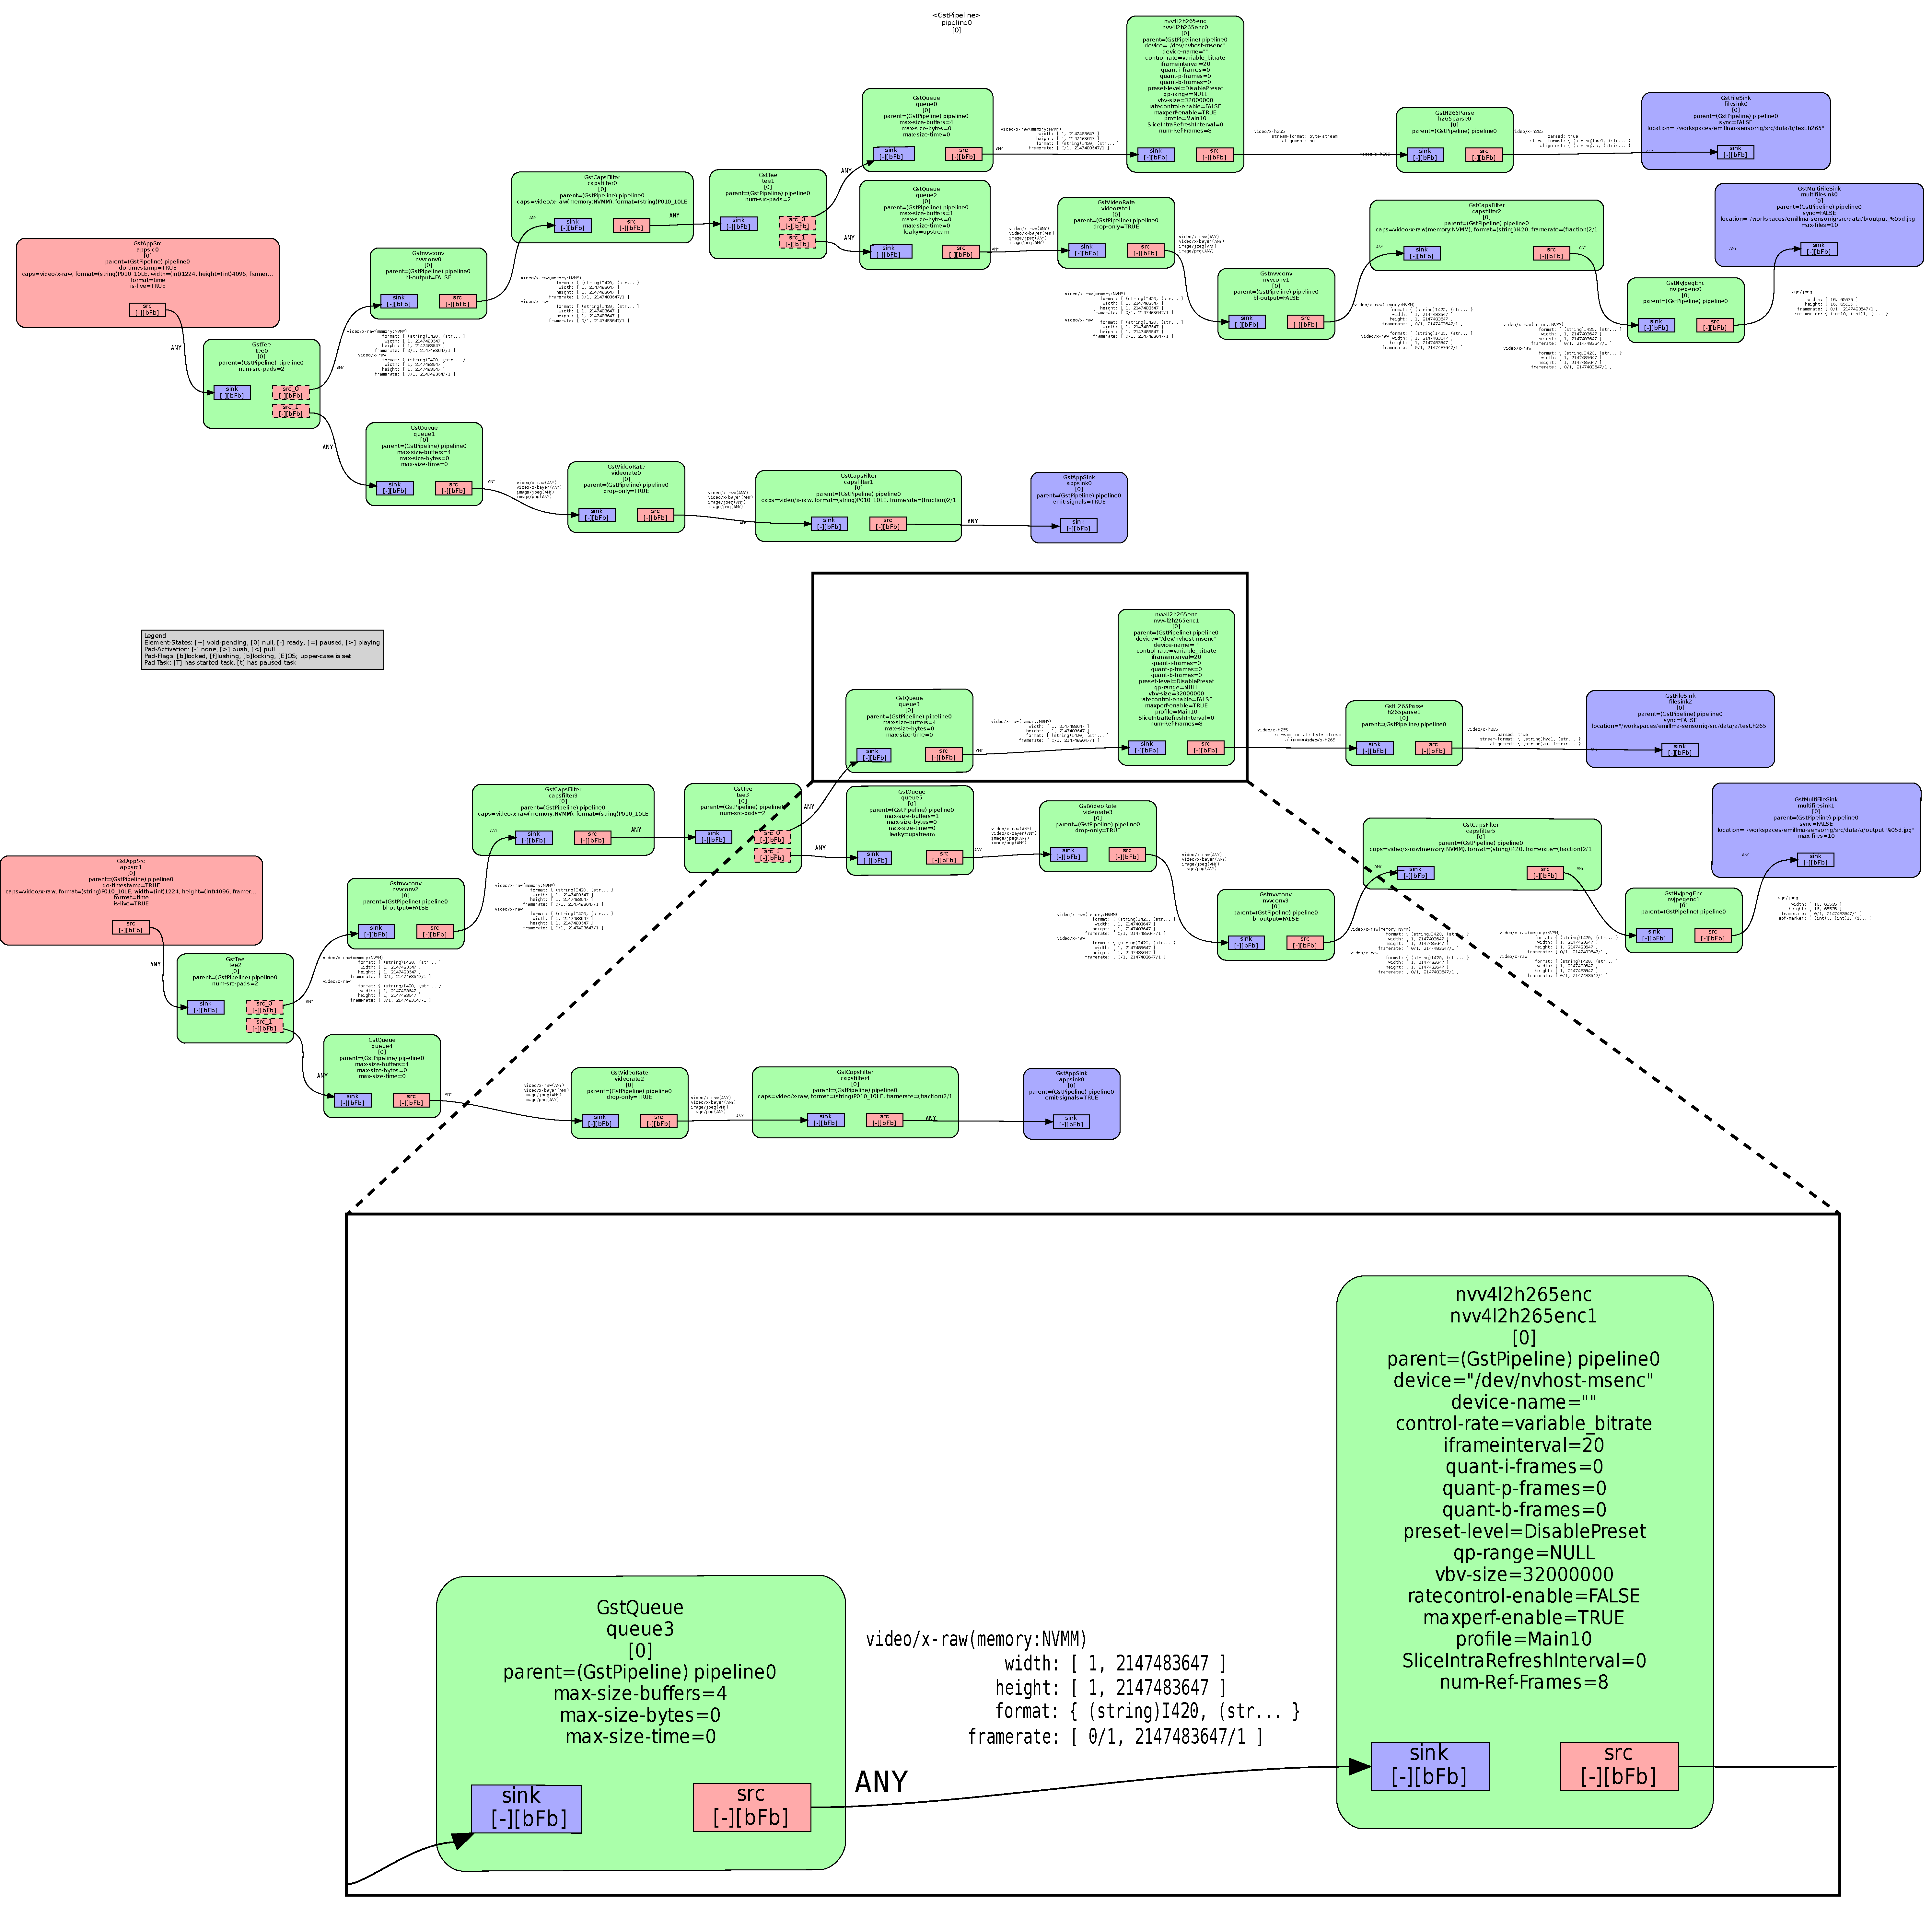
\includegraphics[width=\textwidth]{figures/gstreamer/pipeline.pdf}
    \caption{Visualization of the \gs Pipeline used on the \sr.
        The graph was crated using GraphViz and edited in Adobe Illustrator to be more compbact and readable. The bottom part shows a zoomed in version of the \gls{h265} encoder used on the second camera.}
    \label{fig:gs_pipeline_visualization}
\end{figure}

\subsection{Enabling Debugging of Threads}
The \gls{pygo} appear to runs callbacks in separate Threads.
It was discovered that breakpoints in these threads are ignored by the Debugpy, the default debugger in \gls{vscode} \cite{microsoftDebugpyDebuggerPython2023}\cite{visualstudiocodeDebuggingConfigurationsPython2023}.
Debugging can be enabled manually by calling \code{debugpy.debug_this_thread} at the beginning of the callback function \cite{nadigAnswerDebugNot2019}.


\subsection{Output Inspection}
Reveales use of bt.601 rather than bt.709 color profile.


\begin{figure}[H]
    \centering
    % \begin{tabular}[b]{cc}
    \subcaptionbox{Original frame.}{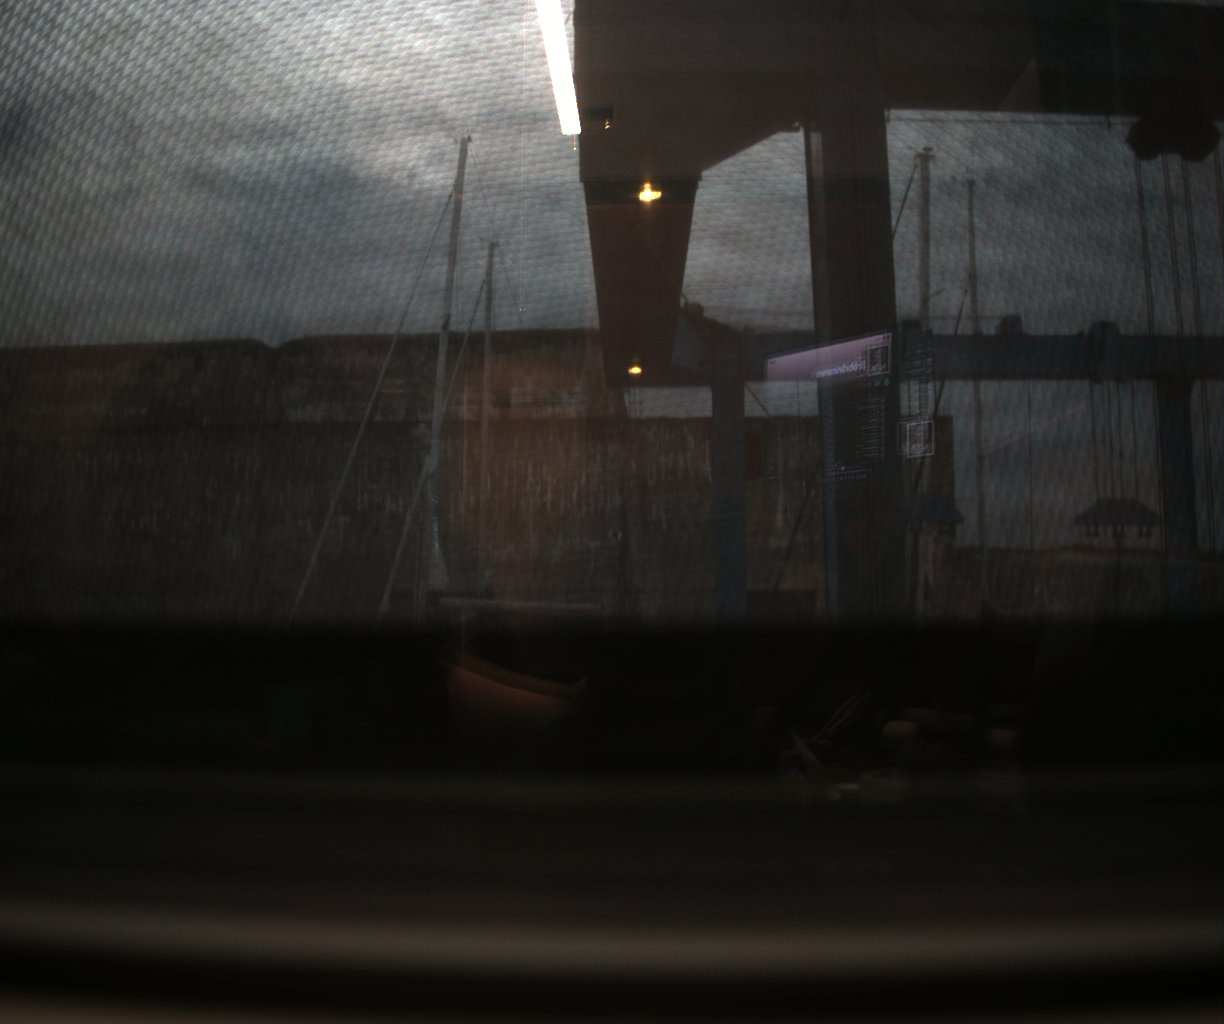
\includegraphics[width=0.48\textwidth]{figures/compression/error_orig.jpg}}
    \subcaptionbox{Original frame subtracted from decompressed frame.}{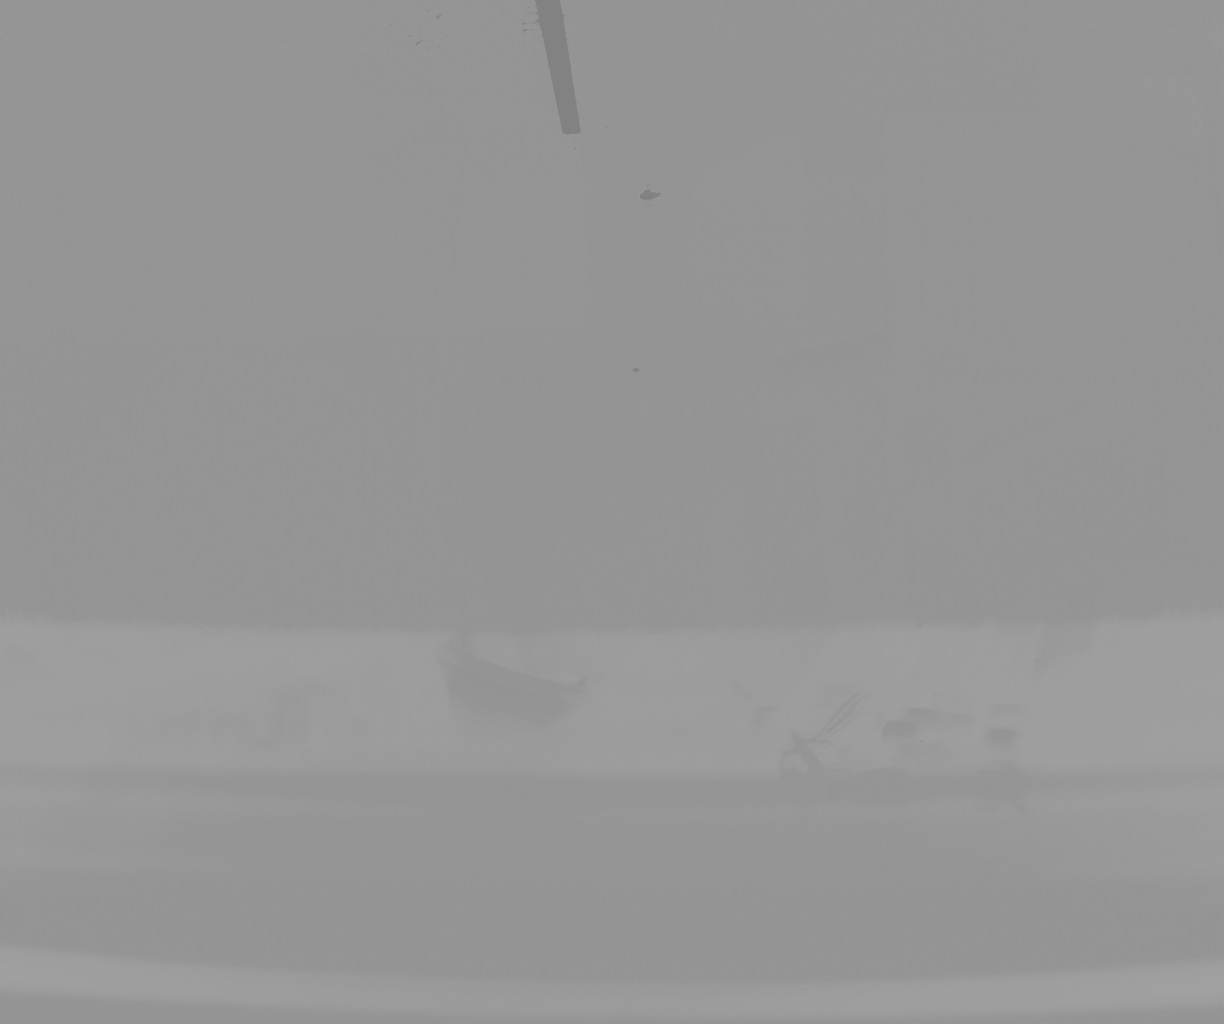
\includegraphics[width=0.48\textwidth]{figures/compression/error_error.jpg}}
    % \end{tabular}
    \caption{Original frame and compression error revealing use of wrong color profile as brigh regions are too dark and dark regions are too bright.}
\end{figure}